%!TEX root = ../lectures_olympics.tex

\chapter{刚体动力学}
过去我们广泛地讨论了质点的运动,当运动物体自身的大小和运动过程中的姿态变化和运动范围或者考察问题的精度相比能够忽略不计时可以当做质点来处理。
但是真实的物体或多或少地占据一定的空间范围,为了更准确地描写物体的运动就必须考虑它所占据的有限体积。
所谓的\emph{刚体}是具有一定形状运动物体的简化模型,它们在其运动过程中形状保持不变,各部分的位置关系一致。
很多真实的物体在一定程度上可以当成刚体来处理,例如天上的飞机、地上的汽车和水中的轮船等等,但必须强调的是这些被当成的刚体的物体在运动过程中实际上形状也会发生变化,例如飞机飞行过程中机机翼会抖动,在颠簸过程中汽车的悬挂系统也会有反应等,但只要这些形变对具体力学问题的研究不重要时就可以将它们当做刚体来处理。
比起质点的运动刚体运动的过程要复杂地多,只需要设想一粒石子和树叶下落过程就能有所体会,这里我们仅学习简单的刚体运动,复杂的运动过程留给大家在随后的过程逐渐掌握。

\section{刚体运动的描写}
因为刚体具有有限的大小,所以为了描写刚体的运动除了需要指出刚体某一时刻所处的位置以外还需要明确地表明它的姿态。
刚体上各部分之间的相对位置永远保持不变,所以刚体的位置可以用它上面任何一点的空间坐标来代表,这些点当中最特殊也最具有代表意义的点自然是刚体的质心或重心,今后统一用刚体的质心来表示刚体的位置。

\begin{example}
试确定以下几个刚体质心的位置:



(a)底面半径为$R$,高为$H$,密度均匀的圆柱体

(b)底面半径为$R$,高为$H$,密度均匀的圆椎体

(c)密度球对称分布的球体,半径为$R$,$r$为一点到球心的距离,密度由函数$\rho(r)$给出。


\tagged{student}{\vspace*{4cm}}
\begin{taggedblock}{teacher}
\noindent
解析:略
\end{taggedblock}
\end{example}
刚体的姿态则需要用通过它质心的三根互相垂直的轴线与空间当中固定的坐标系的坐标轴的夹角来确定,数学上看为了唯一决定刚体的姿态至少需要三个角度,实践上这三个角度的选取具有很大的任意性,今天大家常用的用来规定刚体空间姿态的角度变量称为\emph{欧拉角},图\ref{fig: rg-euler-angle}给出欧拉角的名称和定义。

\begin{figure}[hbtp]

\centering
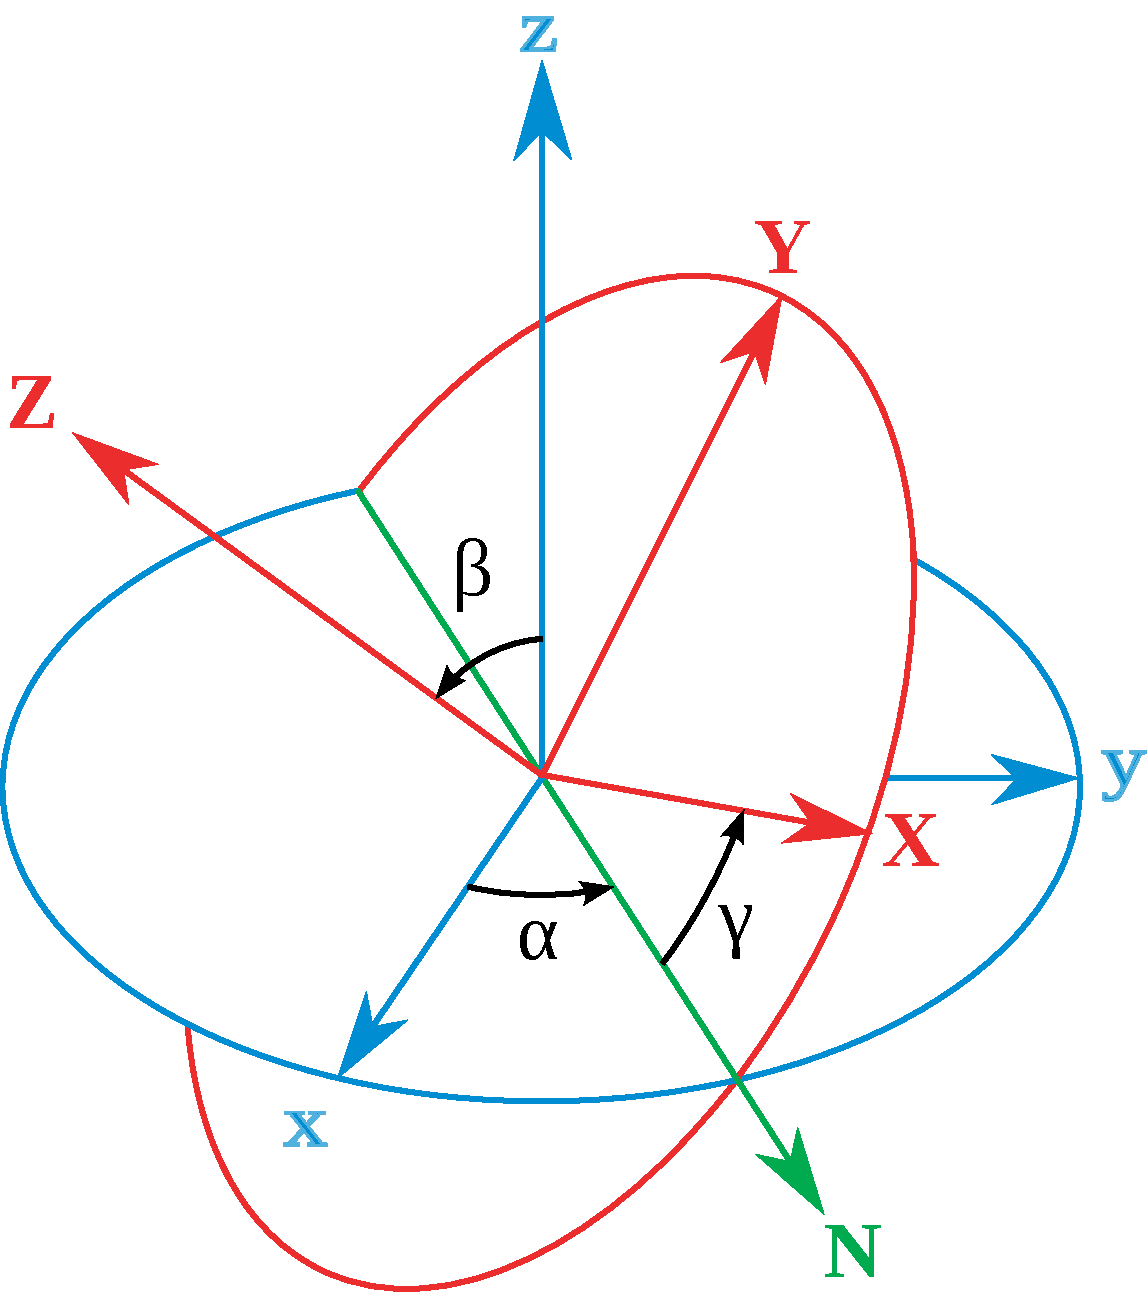
\includegraphics[width=0.5\textwidth]{images/rb-Eulerangles.pdf}
\caption{欧拉角,$xyz$为在固定在空间中的坐标轴,$XYZ$为和固定在刚体的三根轴线,$XYZ$轴可以由$xyz$轴通过一定的转动而得,欧拉角就是一种特定的转动过程所需要转过的角度。}\label{fig: rg-euler-angle}
\end{figure}





一个运动刚体的位置和姿态需要六个运动学变量才能够唯一给出,它们分别是刚体质心的坐标和三个欧拉角,一般的刚体在运动过程中这六个变量都会在外力作用下随时间变化,完整地确定刚体的运动远比质点要复杂地多。
为了不至于陷入过度的数学复杂性,下面我们着重关注几种简单的刚体运动。

\begin{figure}[hbtp]

\begin{minipage}[t]{0.5\linewidth}
\centering
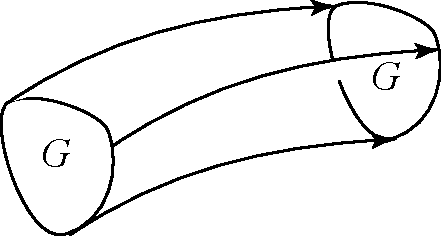
\includegraphics[width=0.8\textwidth]{images/rb-theory-2.pdf}
\caption{平动的刚体}
\label{fig: rb-平动的刚体}
\end{minipage}%
\begin{minipage}[t]{0.5\linewidth}
\centering
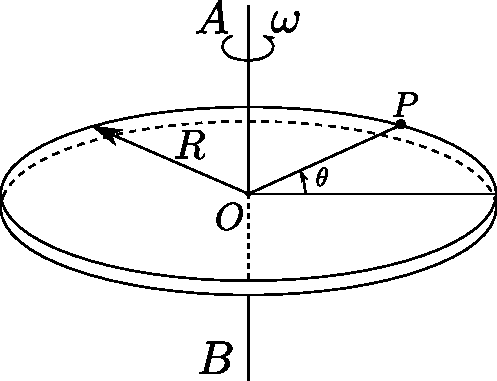
\includegraphics[width=0.8\textwidth]{images/rb-rotation-about-fixed-axis.pdf}
\caption{围绕固定轴线$AB$的定轴转动}
\label{fig: rb-rotation-about-fixed-axis}
\end{minipage}%
\end{figure}
\begin{enumerate}
\item \emph{平动}:如图\ref{fig: rb-平动的刚体}所示,如果一个刚体在运动过程中不发生任何的转动,则称该刚体在作\emph{平动}。
由于各部分相对于质心的位置不发生变化,所以平动刚体的运动可以完全用它质心的坐标来描写。
平动刚体的运动性质和质点没有本质的不同,如果用质心代表刚体的位置,则满足相同的运动定律。

平动刚体在外力作用下同样会做加速运动,满足和质点一样的运动方程:
\begin{equation}
\vec{F} = M\vec{a}_c =M\frac{d\vec{v}_c}{dt} 
\end{equation}
其中$M$为刚体的总质量,速度和加速度加上下标$c$是特指刚体质心的速度和加速度。
和质点一样,运动的刚体同样具有动量和动能,刚体动量和动能为它各部分动量和动能的和,对于平动的刚体来说由于各部分速度的大小和方向都相同,很容易得出平动刚体的动量和动能分别为
\begin{equation}
\vec{p} = M\vec{v}_c,\qquad E_k = \frac{1}{2}Mv_c^2.
\end{equation}

\item \emph{定轴转动}:除了平动以外刚体另外一类简单的运动是围绕一根固定轴线的转动。
图\ref{fig: rb-rotation-about-fixed-axis}给出了最简单的定轴转动的情况,一个刚体圆盘围绕通过它圆心$O$的固定轴线$AB$做定轴转动,转动的角速度为$\omega$。
这时刚体的位置仅由一个变量来决定,例如在刚体上标记一个给定点$P$,它与转轴中心$O$的连线与空间中一个固定方向$Ox$的夹角$\theta$就可以唯一给出转动圆盘所处的位置。
刚体定轴转动的角速度就是角度$\theta$随时间的变化率
\begin{equation}
\omega=\frac{d\theta}{dt}.
\end{equation}



在外力作用下定轴转动的角速度会发生变化,角速度随时间的变化率称为\emph{角加速度},如果用$\beta$来表示角加速度,那么
\begin{equation}
\beta = \frac{d\omega}{dt} = \frac{d^2\theta}{dt^2}.
\end{equation}
外力的效果体现为相对于转动轴的力矩,和通常的定义相同,为力和力臂的乘积,如果有多个力作用于转动刚体时合力矩和单个力存在时力矩的和。
需要特别指出的是和力一样,力矩本质上也是一个矢量,但是对于定轴转动的刚体来说它的矢量性并不明显,只有正负之分。
力矩的正负体现在力的效果使角速度变大或变小,如果力矩有使角速度变大的趋势就称力矩为正,反之为负。
和牛顿第二定律类似的,外力矩$M$将正比于角加速度
\begin{equation}\label{eqn: rb-刚体转动定律}
M = I\beta=I\frac{d\omega}{dt}
\end{equation}
其中比例系数$I$称为\emph{转动惯量},它由刚体的形状、质量分布、转轴的位置和方向共同决定,它是质量在转动情形的推广,是转动物体的一个重要的物理量。

可以把刚体看成的相对距离保持不变的质点构成的复合体,转动刚体的角动量为每个质点围绕固定转轴角动量的和,简单的计算表明定轴转动刚体的角动量为转动惯量与角速度的乘积
\begin{equation}
L = I\omega,
\end{equation}
这样刚体定轴转动的方程\ref{eqn: rb-刚体转动定律}又可以理解成刚体所受力矩为其转动角动量随时间的变化率。
同样的道理,定轴转动刚体的动能为构成刚体的质点动能的代数和,它的大小为
\begin{equation}
E_k = \frac{1}{2}I\omega^2
\end{equation}

\item \emph{滚动}:平稳行驶汽车的轮子就是滚动最简单的例子,滚动的刚体除了有质心的移动的同时还有转动。
当外轮廓为圆的刚体在滚动时,可以用其圆心的速度和围绕圆心转动的角速度一起来描写滚动。
要特别注意两种截然不同的滚动过程:有滑动的滚动和无滑动的滚动。
当沿一条直线滚动刚体球心运动速为$v$,相对质心转动角速度为$\omega$且半径为$R$时,如果$v = \omega R$则刚体作无滑动的滚动,反之当$v\neq \omega R$时则有相对滑动。


\end{enumerate}


\begin{example}
一个质量为$m$的质点和一根质量可以忽略不计、长度为$l$的刚性轻杆构成一个简单的刚体。
质量固定连在杆的一端,整个刚体在通过$O$点垂直于纸面的固定轴转动。
通过牛顿定律证明在任意外力作用下式\ref{eqn: rb-刚体转动定律}的正确性并确定这时转动惯量的值。
\begin{flushright}
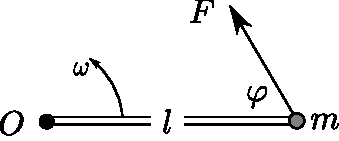
\includegraphics[width = 0.3\textwidth]{images/rb-1.pdf} 
\end{flushright}
\tagged{student}{\vspace*{3cm}}
\begin{taggedblock}{teacher}
\noindent
解析:因为转动的是刚体,所以整个物体的相对位置不会发生变化,设有一个外力$F$它通过$m$与杆的夹角为$\varphi$,$m$只能围绕轴运动,所以只有$F$垂直于杆的分量会对它的运动有影响。
$m$沿垂直于杆的加速度与刚体的角加速度之间的关系可由运动学得到:
\[a = l\beta\]
对于$m$的牛顿第二定律就变成了
\[
F\sin\varphi = ml\beta
\]
两边同时乘以$l$,左边就变成了$F$对转动轴的力矩,而右边则变成
\[ Fl\sin\varphi = M = ml^2\beta = I\beta\]
通过比较马上可得$I=ml^2$。
\end{taggedblock}
\end{example}




\section{转动惯量}
刚体的转动惯量决定了外力矩作用下刚体的运动,是描述刚体运动最重要的物理量之一。
前面我们已经看到,单个质量为$m$的质点当它与转动轴的距离为$l$时,转动惯量$I=ml^2$。
多个质点构成的刚体其转动惯量自然就是每个质点转动惯量之和,设刚体由$N$个质点构成,用自然数$i$来标记各个质点,当质量为$m_i$的质点距离转动轴$l_i$时整个刚体的转动惯量为
\begin{equation}
I = \sum_{i=1}^N m_il_i^2
\end{equation}
更一般地,当刚体是由连续分布的物质构成时,围绕给定轴的转动惯量同样也是各个部分贡献的转动惯量之和,上式的求和也变成了一个积分。

如图所示,一个任意形状的刚体围绕与$z$轴重合的固定轴转动,其各点的密度分布不均匀,用函数$\rho(x,y,z)$表示,这时刚体的转动转动惯量可以表达为
\begin{equation}\label{eqn: rb-刚体转动惯量的一般形式}
I = \int_V \rho(x,y,z)(x^2+y^2)dxdydz
\end{equation}
其中积分区域为整个刚体所占据的空间区域。
对于一般的刚体,利用积分式求它的转动惯量十分复杂,但是如果刚体具有一定的均匀性和对称性的话,就有机会将复杂的积分化为低维的简单积分,可以通过数学计算得到对应情形下转动惯量的准确数值。

\begin{example}
求一根质量为$M$,长度为$l$的均匀细杆绕其中点和端点的转动惯量。
\begin{center}
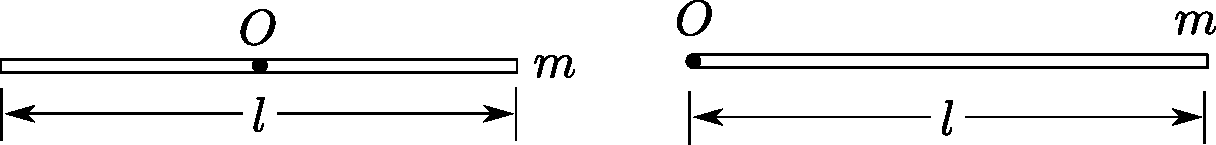
\includegraphics[width=0.7\textwidth]{images/rb-2.pdf} 
\end{center}
\tagged{student}{\vspace*{4cm}}
\begin{taggedblock}{teacher}
\noindent
解析:两种情况下杆的线密度均为$\lambda = M/L$,根据转动惯量的定义两种情况下分别为
\begin{eqnarray*}
I_1 &= &\int_{-L/2}^{L/2}\lambda x^2dx = \lambda\cdot \frac{1}{3}x^3\bigg|_{-L/2}^{L/2} = \frac{M}{L}\cdot \frac{1}{3}\frac{M}{L}\frac{1}{4}L^3 = \frac{1}{12}ML^2\\
I_2 &=&  \int_{0}^{L}\lambda x^2dx = \frac{1}{3}\frac{M}{L}L^3 = \frac{1}{3}ML^2
\end{eqnarray*}
\end{taggedblock}
\end{example}

\begin{example}
求一个质量为$M$,半径为$R$的均匀圆盘围绕通过其圆心垂直于盘面轴的转动惯量。
\tagged{student}{\vspace*{4cm}}
\begin{taggedblock}{teacher}
\newline
解析:圆盘的面积密度为$\sigma = \frac{M}{\pi R^2}$,将圆盘切割成一个个的圆环,每个圆环贡献的转动惯量分别为
\[dI = \frac{M}{\pi R^2}\cdot 2\pi r dr\cdot r^2\]
这样整个圆盘的转动惯量将是上式从0到$R$的积分:
\[
I = \frac{2M}{R^2}\int_0^Rr^3dr = \frac{1}{2}MR^2
\]
\end{taggedblock}
\end{example}


\begin{example}
求一个质量为$M$,半径为$R$的均匀球壳相对其通过球心轴的转动惯量为$\frac{2}{3}mR^2$。
\tagged{student}{\vspace*{4cm}}
\begin{taggedblock}{teacher}
\newline
解析:\[dI = \frac{M}{4\pi R^2}2\pi\cos\theta*Rd\theta*(R\cos\theta)\]
角度$\theta$从$-\frac{\pi}{2}$积分到$\frac{\pi}{2}$
\[I = \frac{MR^2}{2}\int_{-\frac{\pi}{2}}^{\frac{\pi}{2}}\cos^3\theta d\theta=\frac{2MR^2}{3}\]
\end{taggedblock}
\end{example}

当刚体围绕某一特定轴的转动惯量为已知时,沿着平行于该轴的其它轴作定轴转动的惯量其实并不需要重新计算新的积分式。
对于那些由多个质点构成的刚体来说,通过它质心的转动轴非常特殊,假设此时它的转动惯量为$I_{c}$,根据定义可知
\begin{equation}
I_{c} = \sum m_i(x_{ic}^2+y_{ic}^2)
\end{equation}
其中$x_{ic}$、$y_{ic}$分别为质量为$m_i$的质点相对于通过质心轴的$x$、$y$坐标,这里我们假设转动轴和$z$轴重合。
那么对于$x$坐标为$X$的另外一根平行于$z$轴的转动轴来说,质量为$m_i$的质点在以新轴为坐标原点坐标系的坐标值则是
\[x_i = x_{ic}-X,\qquad y_i = y_{ic}\]
这时转动惯量根据定义可以写成
\begin{eqnarray}
I &=& \sum m_i(x_i^2+y_i^2) = \sum m_i((x_{ic}-X)^2+y_{ic}^2)\nonumber\\
&=& \sum m_i (x_{ic}^2+y_{ic}^2)+\sum m_i X^2 -2X\sum m_i x_{ic}\nonumber\\
&=&I_c +MX^2 
\end{eqnarray}
其中$M$为刚体的总质量,倒数第二行最后一项由于质心的性质完全消失。
很容易证明,对于其它平行于通过质心转轴的转动惯量也满足上式,只不过最后一行中的$X$要用新的轴与通过质心轴之间的距离$r$来代替,进一步可以证明上式对于质量连续分布的刚体同样成立。
也就是说刚体沿任意轴的转动惯量$I$等于平行于该轴并通过质心时的转动惯量$I_c$与刚体总质量与两轴距离平方的乘积$Mr^2$之和
\begin{equation}
I = I_c + Mr^2
\end{equation}
这对于任意刚体均成立,称为转动惯量的\emph{平行轴定理}。

另外对于那些厚度可以忽略不计的刚体来说,还有另外一条能够方便地决定转动惯量的定理。
当刚体是由处于一个平面的多个质点构成时,将刚体的平面放置于坐标系中的$xy$平面上,这时通过一个给定点$O$平行与$x$、$y$轴的转动惯量分别为
\[I_x = \sum m_i y_i^2,\qquad I_y = \sum m_i x_i^2\]
而根据定义,通过$O$点垂直于刚体平面的$z$轴的转动惯量则是
\begin{equation}
I_z  = \sum m_i(x_i^2+y_i^2) = I_x+I_y
\end{equation}
这就是刚体转动惯量的\emph{正交轴定理}。
通过平行轴和正交轴定理,并配合对称性可以决定很多规则形状刚体的转动惯量。

\begin{example}
综合利用积分、平行轴和正交轴定理求下列刚体的转动惯量并完成下表





\begin{tabular}{|c|c|c|}
\hline 
物体 & $z$轴 & 转动惯量 \\ 
\hline 
细同心圆环,半径为$r_1$,$r_2$ & 与环垂直,通过中心 &  	 \\ 
\hline 
球,半径为$R$ & 穿过球心 &   \\ 
\hline 
矩形薄片,边长为$a$,$b$ & 与$b$平行,通过中心 &   \\ 
\hline 
矩形薄片,边长为$a$,$b$ & 与薄片垂直,通过中心 &   \\ 
\hline 
薄圆环,半径为$r_1$,$r_2$ & 任一直径 &  \\ 
\hline 
长方形平行六面体,边长为$a$,$b$,$c$&  与$c$平行,通过中心 &    \\ 
\hline 
圆柱体,半径$r$,长度$L$&  与$L$平行,通过中心 &    \\ 
\hline
圆柱体,半径$r$,长度$L$&  与$L$垂直,通过中心 &    \\ 
\hline
\end{tabular} 
\tagged{student}{\vspace*{4cm}}


\begin{taggedblock}{teacher}

\end{taggedblock}
\end{example}

\section{刚体动力学}
当在空间中运动的刚体同时又有转动时问题变得异常复杂,之前对平动和定轴转动为研究一般的刚体运动提供了理论上的基础。
最一般的情况下刚体的运动规律可以总结如下。
无论运动过程中是否发生转动,质心的运动都满足牛顿定律:
\begin{equation}
\vec{F} = M\vec{a}_c
\end{equation}
其中$M$为刚体的质量,$\vec{a}_c$代表其质心的加速度,$F$是刚体所受所有外力的合力。
如果在运动过程中刚体发生转动时,特别注意只有质心的加速度满足上式,无论各个外力的作用点如何。
例如抛出的刚体如果忽略空气阻力,一般来说会翻滚着飞行,尽管它上面普通一点的轨迹可能很复杂,但无论其运动方式如何,质心均无一例外地沿抛物线运动。

当有外力的作用方向不通过质心时会对刚体产生力矩,一般地讲力矩会引起角动量的变化,也就是转动速度的变化。
原则上讲角动量定理对于任意的参考点均成立,但在研究刚体运动时我们特别强调相对于通过质心转轴的角动量定理:刚体所受外力的合力矩等于相对于通过质心轴的角动量随时间的变化率。
选用通过质心的轴利用角动量定律的好处有很多,首先绝大部分典型的外力,尤其是重力必然通过质心,这使得能够贡献通过质心轴力矩的力的数量大大减少,使计算变得容易;更重要的,当刚体的质心本身在作加速运动时,如果不选择通过质心的轴,那么必须考虑惯性力的作
用,增加了分析的复杂性,所以一般来说都选择通过质心的轴来使用角动量定理。

\begin{figure}[htbp]
\begin{center}
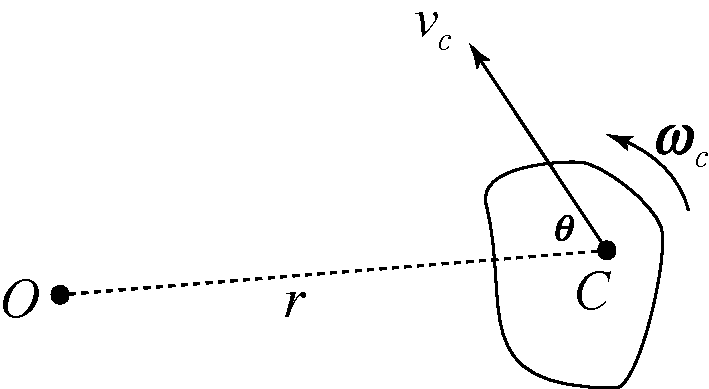
\includegraphics[width=0.5\textwidth]{images/rb-theory-1.pdf}
\caption{一般运动刚体的角动量可以分解为质心的角动量和相对于质心转动角动量的和}
\label{fig: rb-general-angular-momentum}
\end{center}
\end{figure}


利用质心的性质,刚体运动过程中的动力学变量也能够得到极大的简化。
刚体相对于空间中一给定点的角动量同样是构成刚体各部分对同一点角动量之和,可以证明它可以简化为刚体质心的角动量以及相对于质心转动角动量之和,如图\ref{fig: rb-general-angular-momentum}所示,当刚体质心速度为$v_c$,相对质心转动惯量为$I_c$、角速度为$\omega_c$时,且转动轴垂直于刚体质心与$O$的连线以及质心速度所决定的平面时,相对$O$点的角动量
\begin{equation}\label{eqn: rb-刚体一般动量}
L_o = Mv_cr\sin\theta + I_c\omega_c,
\end{equation}
其中$\theta$角为质心的速度与$OC$连线方向的夹角。
一个简单的例子就是地球相对于太阳的角动量为其公转角动量和自转角动量之和。
同理刚体的动能也可写为质心的动能和相对于质心转动动能的和:
\begin{equation}\label{eqn: rb-刚体一般动能}
E_k = \frac{1}{2}Mv_c^2+ \frac{1}{2}I_c\omega_c^2,
\end{equation}
其中$M$为刚体的总质量,$v_c$为质心运动速度,$I_c$为通过质心轴的转动惯量,$\omega_c$则是相对于质心转动的角速度。

\begin{example}
一个简单的刚体由两个质量$m$相等的质点之间由长度为$l$、质量忽略不计的杆连接。
在某一时刻它质心的速度为$v$,垂直于杆的方向,相对质心转动的角速度为$\omega$,其方向如图所示。
定义角动量的参考点$O$刚好位于杆的连线方向,与杆中点的距离为$L$。
请验证刚体相对于$O$点的角动量以及刚体的动能分别满足\ref{eqn: rb-刚体一般动量}、\ref{eqn: rb-刚体一般动能}。
\begin{flushright}
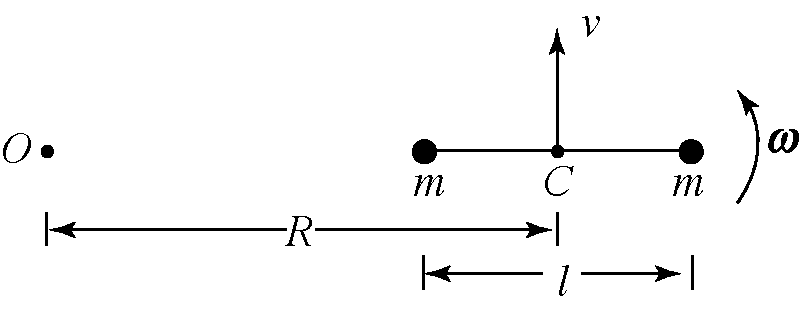
\includegraphics[width=0.4\textwidth]{images/rb-problem-5.pdf}
\end{flushright}
\tagged{student}{\vspace*{2cm}}
\begin{taggedblock}{teacher}
\noindent
解析:略
\end{taggedblock}
\end{example}

\begin{example}
一个转动惯量为$I$的刚体在大小不变的外力矩$M$作用下,初始时刻$t=0$的角速度为$\omega_0$,角度为$\theta_0$,求此后刚体的角速度、角位置随时间的关系$\omega(t)$和$\theta(t)$。
\tagged{student}{\vspace*{4cm}}
\begin{taggedblock}{teacher}
\newline
解析:和质点的匀加速运动的方程类比即可,此时刚体的角加速度为定值
\[\beta = \frac{M}{I}\]
这时给定初始条件的刚体运动方程为
\[\omega(t) = \omega_0+\beta t,\qquad \theta(t) = \theta_0+\omega_0 t+\frac{1}{2}\beta t^2,\]
这里特别要强调的是角度、角速度以及力矩不但有大小,还有方向。
\end{taggedblock}
\end{example}

\begin{example}
将一个质量为$M$刚体悬挂于通过刚体上$O$点且垂直于纸面的固定轴上,这时以$O$为转轴刚体的转动惯量为$I$,其质心$C$与$O$点相距$l$,证明刚体作微幅摆动的周期
\[T = 2\pi\sqrt{\frac{I}{Mgl}}.\]
\begin{flushright}
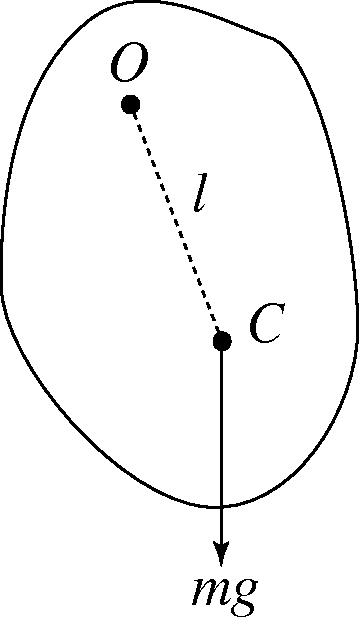
\includegraphics[width=0.2\textwidth]{images/rb-problem-7.pdf}
\end{flushright}
\tagged{student}{\vspace*{2cm}}
\begin{taggedblock}{teacher}
\noindent
解析:略
\end{taggedblock}
\end{example}


\begin{example}
通过受力分析证明,在粗糙的地面上作无滑动滚动刚体与地面之间无摩擦力。
\tagged{student}{\vspace*{4cm}}
\begin{taggedblock}{teacher}
\newline
解析:略
\end{taggedblock}
\end{example}


\begin{example}
有一个长度为$L$,倾角为$\theta$的粗糙斜面,在其顶端有一个质量为$m$,半径为$R$外轮廓为圆形的刚体由静止开始下滚,该刚体的质心位于圆心,围绕通过圆心轴的转动惯量为$I$。
已知在下滚过程中刚体始终作无滑动的滚动

(1)求其下滚过程中质心的加速度,滚动到斜面底部所用的时间,到达斜面底部时质心的速度以及相对于质心转动的加速度。

(2)如果斜面和刚体之间的摩擦系数为$\mu$,如果能够实现上述过程,求$\mu$需要满足的条件。

(3)在斜面和刚体之间的摩擦系数$\mu$太小无法实现无滑动滚动的情况下,重新求解第(1)问中的各个物理量。

\begin{flushright}
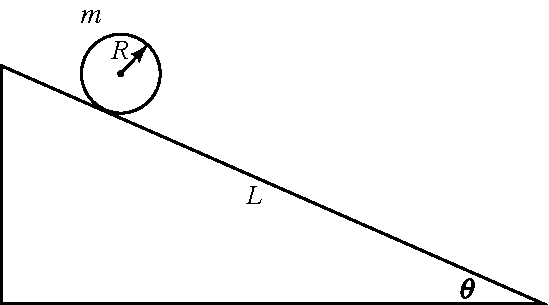
\includegraphics[width=0.4\textwidth]{images/rb-problem-1.pdf}
\end{flushright}
\tagged{student}{\vspace*{4cm}}
\begin{taggedblock}{teacher}
\noindent
解析:(1)设加速度为a,角加速度为$\beta$ \[mg\sin\theta-f=ma,fR=I\beta,\beta R=a\]
解出\[a=\frac{g\sin\theta}{1+\frac{I}{mR^2}}\]
然后很容易计算到达底部时质心的速度了。
(2)第一问中的摩擦力\[f=mg\sin\theta*\frac{\frac{I}{mR^2}}{1+\frac{I}{mR^2}}\]
  条件是:\[\frac{f}{mg\cos\theta}\ge\mu\]
(3)与第一问不同,三个方程变为:\[f=mg\mu\cos\theta,mg\sin\theta-f=ma,fR=I\beta\]

\end{taggedblock}
\end{example}

\begin{example}
在水平面上有一个密度均匀,质量为$m$,半径为$R$,与平面之间摩擦系数为$\mu$的实心球,在$t=0$时受到通过质心的冲击,使质心获得了初速度$v_0$,相对质心转动的角速度为零。
物理的分析和生活经验都表明,最终在摩擦力的作用下它将到达无滑动的滚动状态。
求到达无滑滚动状态所需要的时间、球走过的距离、无滑滚动时质心的线速度以及整个过程中由于摩擦力而损失的动能。
已知均匀球体相对于通过质心轴的转动惯量$I=\frac{2}{5}mR^2$。
\begin{flushright}
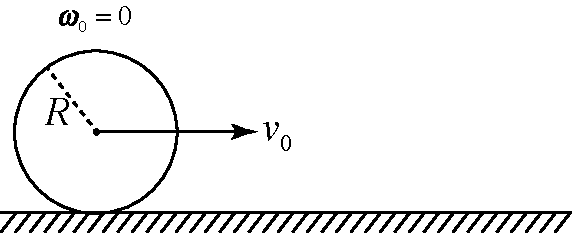
\includegraphics[width=0.4\textwidth]{images/rb-problem-2.pdf}
\end{flushright}
\tagged{student}{\vspace*{4cm}}
\begin{taggedblock}{teacher}
\noindent
解析:$t=\frac{2v_0}{7g\mu},s=\frac{12v_0^2}{49},v=\frac{5v_0}{7},\Delta E=\frac{mv_0^2}{7}$
\end{taggedblock}
\end{example}


\begin{example}
在水平面上有一个密度均匀,质量为$m$,半径为$R$,与平面之间摩擦系数为$\mu$的实心球,在$t=0$其质心速度为零但具有非零的角速度$\omega_0$,在摩擦力的作用下它将向前滚动并最终达到无滑滚动状态,求此过程所需要的时间、球走过的距离、无滑滚动时质心的线速度以及整个过程中由于摩擦力而损失的动能。
已知均匀球体相对于通过质心轴的转动惯量$I=\frac{2}{5}mR^2$。
\begin{flushright}
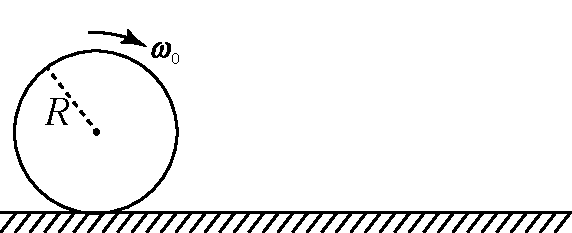
\includegraphics[width=0.4\textwidth]{images/rb-problem-3.pdf}
\end{flushright}
\tagged{student}{\vspace*{4cm}}
\begin{taggedblock}{teacher}
\noindent
解析:$t=\frac{2\omega_0R}{7g\mu},s=\frac{2\omega_0^2R}{49},v=\frac{2\omega_0R}{7},\Delta E=\frac{m\omega_0^2R^2}{7}$
\end{taggedblock}
\end{example}


\begin{example}
在水平面上有一个密度均匀,质量为$m$,半径为$R$,与平面之间摩擦系数为$\mu$的实心球,在$t=0$其质心速度为$v_0$且具有向后转动的角速度$\omega_0$

(1)这个游戏很多同学都玩过,当向后转动的角速度足够大时球最终将向后运动,求最终能够实现向后运动角度速度的临界值$\omega_c$

(2)如果最终能够向后运动,求最终向后滚动的速度以及向前运动的最远距离。

已知均匀球体相对于通过质心轴的转动惯量$I=\frac{2}{5}mR^2$。
\begin{flushright}
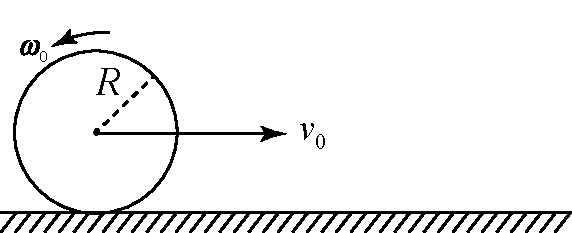
\includegraphics[width=0.4\textwidth]{images/rb-problem-4.pdf}
\end{flushright}
\tagged{student}{\vspace*{4cm}}
\begin{taggedblock}{teacher}
\noindent
解析:(1)$\omega_0=\frac{5v_0}{2R}$
\\(2)$v=R(\omega_0-\frac{5g\mu}{2R}t)=g\mu t-v_0$ 解出:$v=\frac{2\omega_0R-5v_0}{7}$
\\最远的时候$t=\frac{v_0}{g\mu}$,平动速度为0,向前运动的距离最远达到:$\frac{v_0^2}{2g\mu}$
\end{taggedblock}
\end{example}

\begin{example}
在水平面上有一个密度均匀,质量为$m$,半径为$R$,与平面之间摩擦系数为$\mu$的实心球,在$t=0$其质心速度为$v_0$且具有向后转动的角速度$\omega_0$,在其初速度方向正前方$L$处有另外一个完全相同的静止的球。

(1)给出第一个运动的球能够撞上静止球的条件

(2)如果能够相撞,在撞前一瞬间球分别处于无滑动滚动、有滑动的向前转动、有滑动的向后转动状态时,各个已知量分别需要满足的条件。
\begin{flushright}
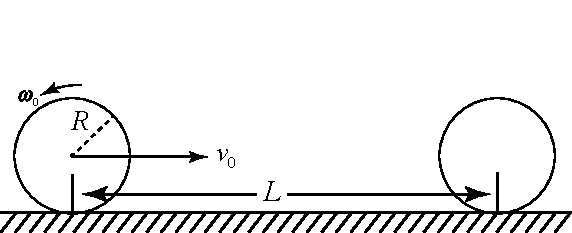
\includegraphics[width=0.4\textwidth]{images/rb-problem-6.pdf}
\end{flushright}

\tagged{student}{\vspace*{4cm}}
\begin{taggedblock}{teacher}
\noindent
解析:(1)$\frac{v_0^2}{2g\mu}=L$
\\(2)略
\end{taggedblock}
\end{example}

